%\documentclass{report}
%\usepackage[T1]{fontenc}
%\usepackage[utf8]{inputenc}
%\usepackage[francais]{babel}
%\usepackage{amsmath}
%\usepackage{graphicx}
%\graphicspath{{Figures/}}
%\usepackage[backend=biber,style=authoryear,bibencoding=utf8]{biblatex}
%\usepackage[colorlinks,linkcolor=blue]{hyperref}
%\newcommand{\micro}{$\mathrm{\mu}$}
%
%\begin{document}

\chapter{Rhéologie locale d'une cellule unique}

Les pinces magnétiques ont été construites afin de pouvoir observer l'évolution des caractéristiques mécaniques d'une cellule au cours du temps, lorsque celle-ci est soumise à des forces de manière répétée. L'objectif était de poursuivre ainsi une investigation débutée par Delphine Icard avec les pinces optiques. En effet, dans sa thèse, elle avait observé que lorsqu'une force identique est appliquée de manière répétée sur une cellule, elle devient de plus en plus rigide, et que cet effet s'accompagne d'un recrutement d'actine autour du point d'application de la force. 

Deux expériences sont décrites ici : les expériences faites avec la pince immédiatement après sa construction et donc le but est d'observer l'évolution des paramètres mécaniques de C2C12 isolées, et des expériences faites bien après en collaboration avec Pierre-Oliver Strale sur d'autres cellules exprimant des cadhérines mutantes. 

\section{Description}

\subsection{Séries d'expériences}

Trois séries d'expériences ont été réalisées avec les pinces magnétiques.
La première série d'expérience a été réalisée sur des C2C12 en testant deux concentrations de fibronectine pour enrober les billes magnétiques : 2 \micro g ou  4 \micro g de fibronectine pour $2.10^7$ billes, ce qui correspond à 1.57 et 3.15 mg/m$^2$ de fibronectine par unité de surface des billes. 
On applique sur ces cellules 4 créneaux de force successifs de 125 secondes chacun avec une période de 250 secondes. 

La seconde série d'expériences a été réalisée sur une autre série de C2C12, issues d'une nouvelle commande à l'ATCC, 4 \micro g de fibronectine sur $2.10^7$ billes et 6 fois 125 secondes de force avec une période de 250s. 
À la suite des expériences de la série \no 1, il nous est en effet apparu que 4 applications de force ne permettaient pas toujours de caractériser le comportement à long terme de la cellule, et nous avons donc augmenté le nombre d'applications de force. 

La troisième série d'expériences est un témoin réalisé avec les mêmes cellules que l'expérience précédente, la même quantité de fibronectine sur les billes, mais seulement 10 secondes d'application de la force, ce qui correspond au temps nécessaire pour extraire les paramètres mécaniques de la cellule. 


Enfin les pinces magnétiques ont également servi à faire des mesures dans le cadre d'une collaboration avec Pierre-Olivier Strale et René-Marc Mège de l'Institut Jacques Monod. Il s'agissait de mesurer les caractéristiques mécaniques de cellules A431D exprimant une cadhérine mutante incapable de former des interactions cis avec d'autres cadhérines de la même membrane, et des billes enrobées de cadhérines et non de fibronectine. 


\subsection{Sélection préliminaire}

Une fois l'expérience mise en place comme cela a été décrit dans le chapitre précédent, la première étape consiste à trouver une bille adhérent à une cellule sur laquelle on puisse faire des mesures. 
On écarte volontairement toutes les billes qui sont trop proches d'une autre bille : en effet, lorsque deux billes sont proches, elles interagissent, et s'attirent l'une vers l'autre jusqu'à former un doublet aligné avec les lignes de champ magnétiques. Il est alors impossible de connaître précisément la force exercée sur la bille. 

Lorsque l'on repère une bille isolée adhérent à une cellule, un premier test rapide est réalisé.
On commence par appliquer une force oscillante sur la bille, et on observe si un mouvement oscillant de la bille est détectable. Si aucun mouvement n'est détectable, on augmente la force jusqu'à détecter un mouvement. Si aucun mouvement n'est détectable à la force maximale, c'est que la bille est trop fortement ancrée, et la cellule trop rigide pour que l'on puisse mesurer ses caractéristiques à l'aide de notre dispositif. 

Il aurait été intéressant de compter le nombre de cellules écartées à cause d'une trop grande rigidité, car cela nous aurait donné un aperçu de la quantité de la population qu'il était impossible de sonder avec le dispositif tel qu'il était monté. Cela a d'ailleurs été fait dans la deuxième expérience sur les cadhérines mutées. 

\subsection{Sélection a posteriori}

Il arrive qu'au cours de l'expérience, lorsqu'une bille n'est que peu ancrée à la cellule, elle soit arrachée lors d'une application de la force.
Il peut également arriver que la cellule observée ait un mouvement propre tellement important qu'elle fait sortir la bille du  champ de la caméra. 

Dans ces deux cas, les expériences partielles ne sont pas dépouillées avec les autres, car il leur manque une partie de l'information, mais elles sont dénombrées.

\subsection{Application de la force : la fonction de fluage}

\subsubsection{Direction du mouvement des billes}
Au temps t=0, une force constante est appliquée sur la cellule par l'intermédiaire de la bille. 

La bille est attirée par la pointe de la pince par une force $\vec{F_{tot}}=F \vec{u}_x+F\vec{u}_z$ dirigée selon l'axe bille-pointe. 

Sur la vidéo, on peut observer la position dans le plan XY du centre de la bille, et constater que la bille est bien attirée par la pointe selon X et n'a qu'un mouvement faible selon Y dû aux petits défauts d'alignement de la pointe. La plupart des billes ont un mouvement total de l'ordre de 0.1 à 0.5 \micro m lors d'une application de force. 

Une fois les positions du centre de la bille extraites de la vidéo par le logiciel d'analyse d'images, on peut en tirer le déplacement de la bille par rapport à sa position au temps t=0 de l'application de la force, pour chaque créneau. 
 

On peut également obtenir des information sur le mouvement de la bille en Z en observant la variation de son rayon, qui augmente lorsqu'elle quitte le plan focal. 

Une calibration à l'aide d'une cale piézo-électrique a permis de déterminer qu'une variation de diamètre de la bille de 0.04\micro m correspond à une variation de hauteur de 0.2 \micro m. 
Or sur la quasi-totalité des billes observées au cours de ces expériences, la variation du diamètre des billes est inférieure à 0.02 \micro m, ce qui correspond à une borne supérieure de mouvement vertical de 0.1 \micro m de l'ordre de la borne inférieure des mouvements détectés selon l'axe X. 

La pince magnétique applique une force égale selon les deux axes X et Z, mais les déplacements mesurés dans les deux directions sont différents : les cellules semblent plus rigides dans la direction verticale par rapport à l'horizontale. 

A AJOUTER : CELLULES DE PIERRE-OLIVIER QUI BOUGENT PLUS EN VERTICAL : CELLULES PLUS EPAISSES ? 


\subsubsection{Fonction de fluage en loi de puissance}

Par défaut, la fonction de fluage sera calculée sans son préfacteur géométrique, qui dépend du modèle choisi mais est strictement identique d'une expérience à l'autre ici.
$$ J(t) = 2 \pi a p \xi (t)\qquad \xi (t) = \frac{\delta R (t)}{F}$$
	
\begin{figure}
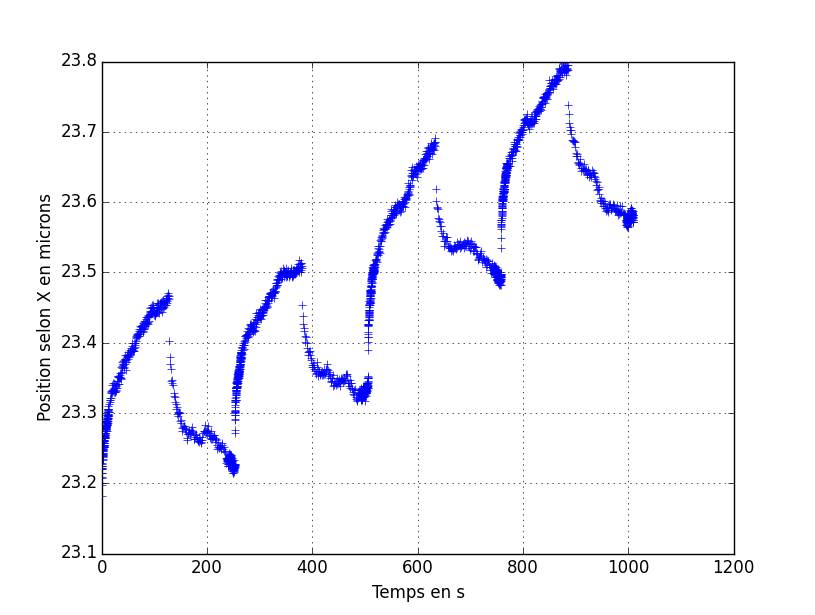
\includegraphics[scale=0.5]{Figures/Exemple_C162_X_vs_slice.png}

\caption{Exemple de tracé de la position en X d'une bille au cours du temps lorsqu'elle est soumise à 4 créneaux de force successifs. $\delta R(t)$ est directement proportionnelle à $\delta X(t)$ lorsque le déplacement ne se fait que selon l'axe $X$. On peut remarquer l'allure caractéristique en loi de puissance.\label{Exemple}} 
	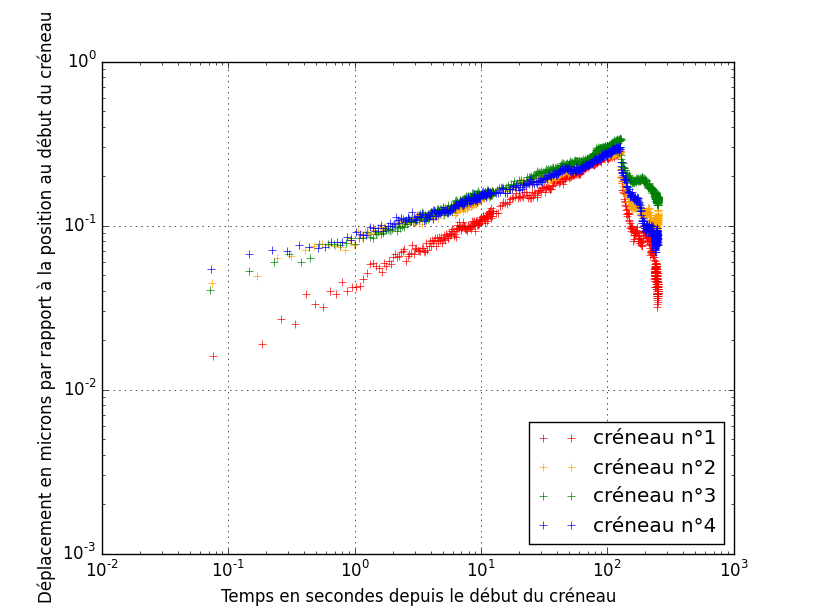
\includegraphics[scale=0.5]{Figures/Exemple_C162_loglog.png}
	\caption{Déplacement de la bille en fonction du temps écoulé depuis le début du créneau, pour les 4 créneaux successifs, pour la même cellule que la figure \ref{Exemple}. On peut remarquer ici qu'après le premier créneau le déplacement est plus grand en réponse à la même force : la cellule s'est ramollie. }
\end{figure}

	 
La fonction de fluage de la cellule peut être modélisée par une loi de puissance à une échelle de temps inférieure à 15-20 secondes. Au-delà, les mouvements actifs de la cellule perturbent le mouvement de la bille. 

On peut alors réaliser un ajustement avec la fonction : 
$$ \xi (t) = \frac{\delta x}{F}=A \left( \frac{t}{t_0} \right)^{\alpha}$$

$A$ et $\alpha$ sont les caractéristiques mécaniques de la cellule, $t$ le temps écoulé depuis le début de l'application du pas de force, $t_0$=1s. 

Pour un solide parfaitement élastique, la déformation en réponse à un palier de force est immédiate et constante au cours du temps, et la fonction de fluage est alors l'inverse du module d'Young.
$$J(t)=\frac{1}{E} = 2 \pi a p \xi(t)$$
 $$J_0=\frac{1}{E} = 2 \pi a p A$$
 $$\alpha=0$$
 
 Pour un liquide parfaitement visqueux, la fonction de fluage est alors  proportionnelle au temps écoulé depuis le début de l'application de la force : 
 $$ J(t)=\frac{t}{\eta} = 2 \pi a p \xi(t)$$
 $$J_0=\frac{t_0}{\eta} = 2 \pi a p \frac{A}{t_0}$$
 $$\alpha=1$$
 
 $A$ représente alors la déformabilité du matériau : plus il est élevé à un instant donné, plus le matériau a été déformé à force égale. 
 $\alpha$ quantifie la dépendance temporelle de cette déformation : plus il est grand, plus le matériau aura tendance à couler comme un liquide visqueux, plus il est petit et plus il se déformera comme un solide élastique. 

Un même créneau de force est appliqué 4 à 6 fois sur les billes avec une période de 250 secondes. 
À chaque application de force, on peut extraire les paramètres $A$ et $\alpha$ et ainsi observer leur évolution au cours du temps. 


\section{Résultats}



\subsection{Caractéristiques mécaniques des C2C12}

Les C2C12 sont des cellules très diverses dans leur taille et dans leur forme, mais également en ce qui concerne les paramètres mécaniques : $A$ s'étale sur deux décades, de $7\dot 10^{-5}$ à $9\dot 10^{-3}$ \micro m/pN avec une médiane à $1.22 \dot 10^{-3}$ \micro m /pN.  Avec le modèle de Gallet, cela correspond à des modules visco-élastiques $G_0$ allant de 12 Pa à 6 kPa avec une médiane à 87 Pa. 
Avec le modèle de Kamgoué-Ohayon, on obtient un module d'Young E allant de 4 à 546 Pa, avec une médiane à 32 Pa. 

L'exposant médian, $\alpha=0.18$ nous indique que la réponse mécanique des cellules est principalement élastique ce qui peut nous conforter quant à l'opportunité de cette hypothèse du modèle de Kamgoué-Ohayon.


\begin{figure}
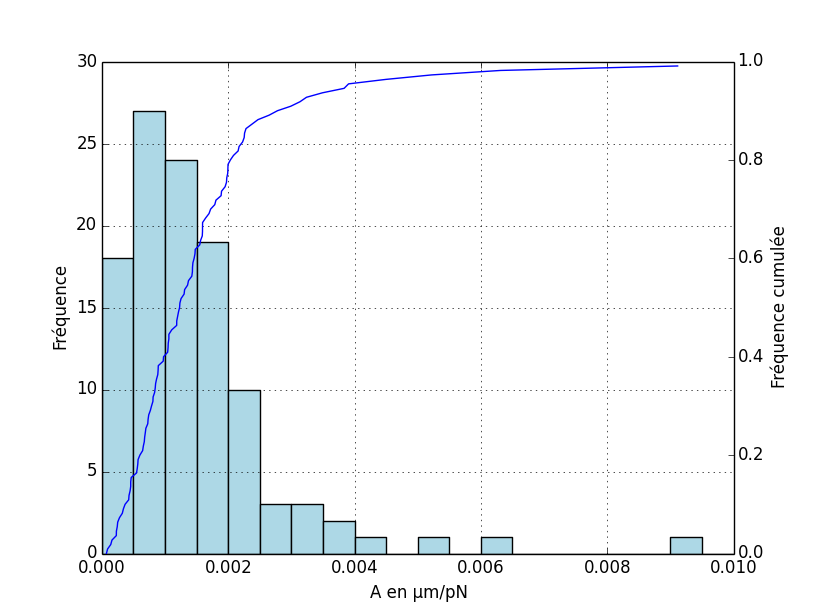
\includegraphics[scale=0.5]{Figures/A0_Toutes.png} 
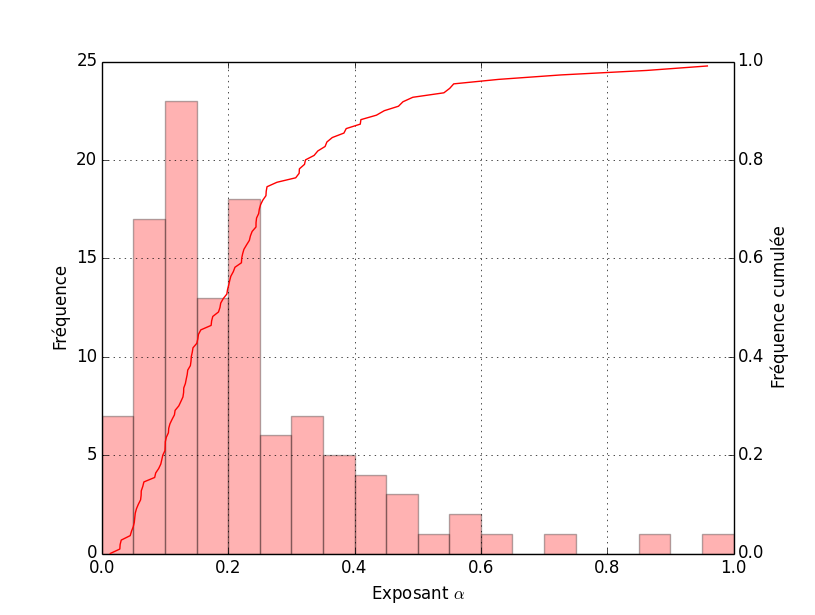
\includegraphics[scale=0.5]{Figures/E0_Toutes.png} 
\caption{Caractéristiques mécaniques des C2C12 avec une concentration de fibronectine disponible sur les billes égale à 3.15 mg/m$^2$}
\end{figure}
 
  
Il est important de rappeler que la population est tronquée de ses cellules les plus rigides, ce qui explique la forme non symétrique de $A$. 
Les valeurs obtenues peuvent paraître faibles en comparaison de celles obtenues précédemment sur la même lignée par Delphine Icard et Elisabeth Charrier, cependant, il est à noter que les angles d'enfoncement choisis ici sont bien plus élevés que les hypothèses retenues dans ces deux autres séries de mesures. De manière générale, on voit que les valeurs de modules visco-élastiques sont très variables d'un modèle à l'autre. 

\subsection{Influence de l'enrobage des billes en fibronectine}

Pendant la première série d'expériences, des billes enrobées de deux concentrations différentes de fibronectine ont été utilisées. 

On peut voir en observant les deux populations que $A$ est plus élevé lorsque l'enrobage est moins dense, alors que l'exposant ne varie pas, mais cette élévation n'est pas significative avec la quantité de cellules que nous avons observées.
Lorsque la quantité de fibronectine sur les billes est plus faible, les cellules apparaissent donc comme plus déformables, moins rigides, ce qui s'explique facilement par un ancrage moindre de la bille au cytosquelette de la cellule.  

En revanche, l'équilibre entre l'élasticité et la dissipation dans la cellule n'est pas altéré : on sonde toujours le même cytosquelette, mais avec un attachement moins fort. 

\begin{figure}
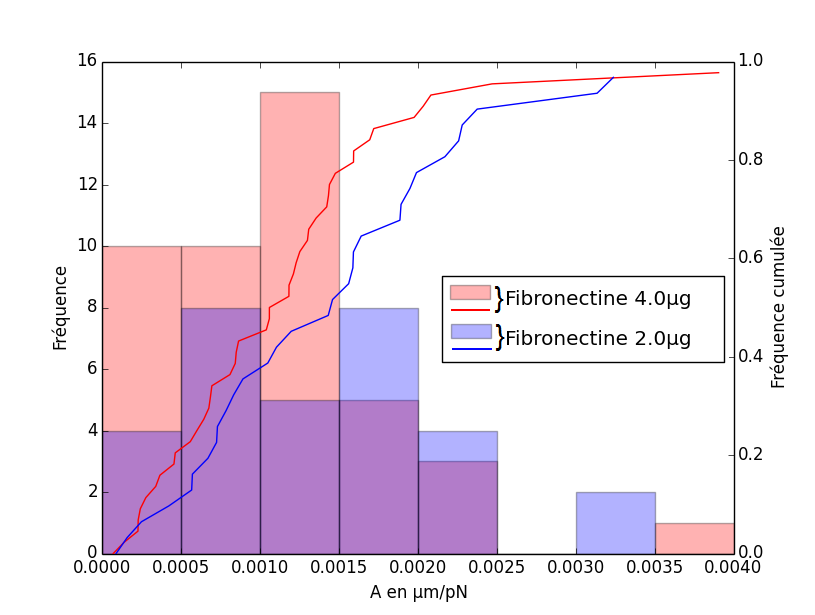
\includegraphics[scale=0.5]{Figures/A_coating.png} 
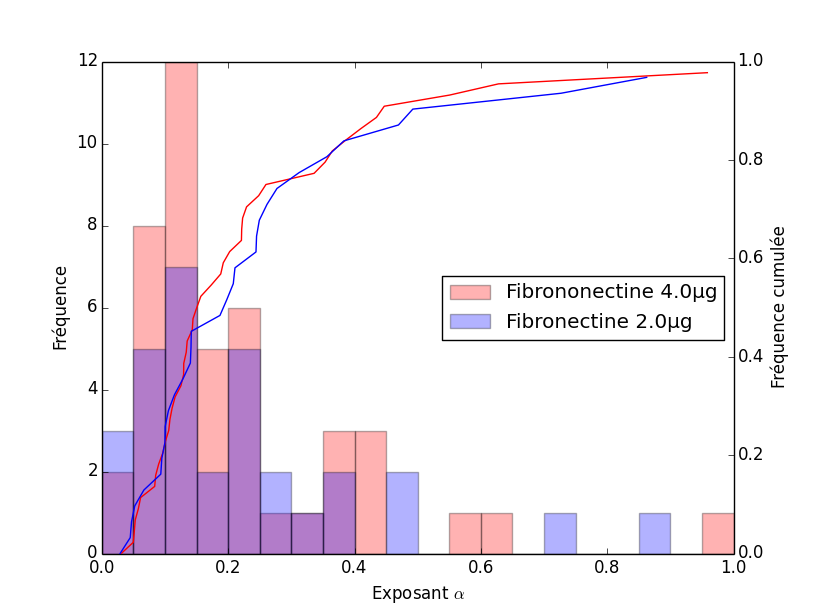
\includegraphics[scale=0.5]{Figures/E_coating.png} 
\caption{Caractéristiques des C2C12 sondées par des billes ayant différentes densités de fibronectine à leur surface. p=0.13}
\end{figure}

\subsection{\'Evolution des paramètres mécaniques}

Pour chaque cellule, la force est appliquée à 4 reprises pour la série \no 1 et à 6 reprises pour les séries \no 2 et \no 3. On obtient alors un coupe de paramètre ($A,\alpha$) par créneau, donc on observe l'évolution. 

Dans les résultats finaux, ne sont conservées que les cellules pour lesquelles la mesure des paramètres ($A, \alpha$) est possible lors de l'application du premier créneau. 
En revanche, il arrive pour un nombre non négligeable de cellules que le déplacement de la bille pendant les créneaux suivants passe en dessous de notre résolution, ce qui signifie que la cellule devient trop rigide. Dans ce cas de figure, $A$ a été fixé à 0. 

\begin{figure}
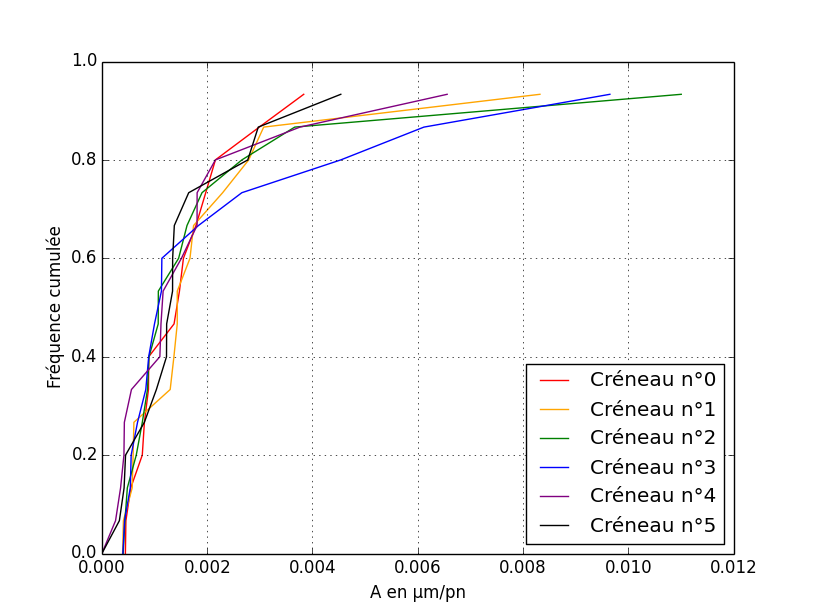
\includegraphics[scale=0.3]{Figures/A_créneaux_témoin.png}
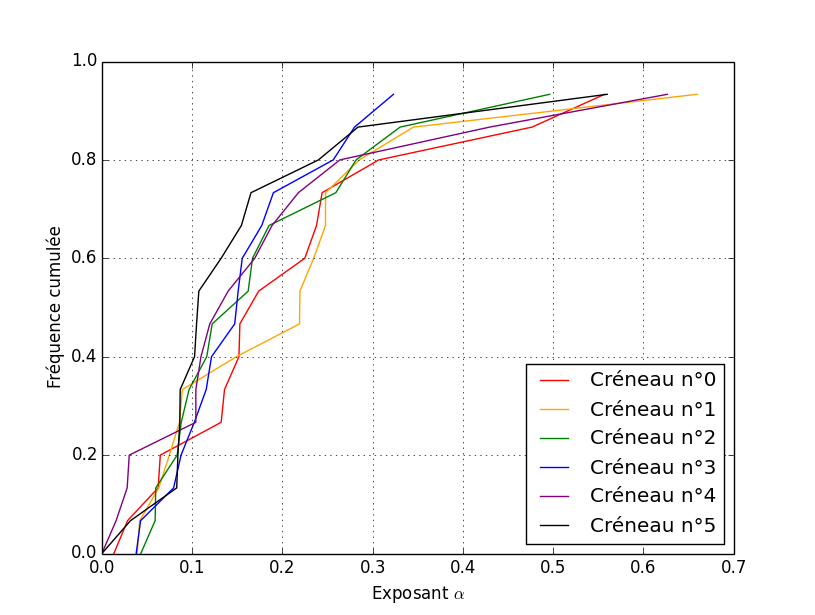
\includegraphics[scale=0.3]{Figures/E_créneaux_témoin.png} 
\\
\includegraphics[scale=0.3]{Figures/A_créneaux_S2.png} 
\includegraphics[scale=0.3]{Figures/E_créneaux_S2.png} 
\caption{\label{Evolution_6c}} 
\end{figure}

\begin{figure}
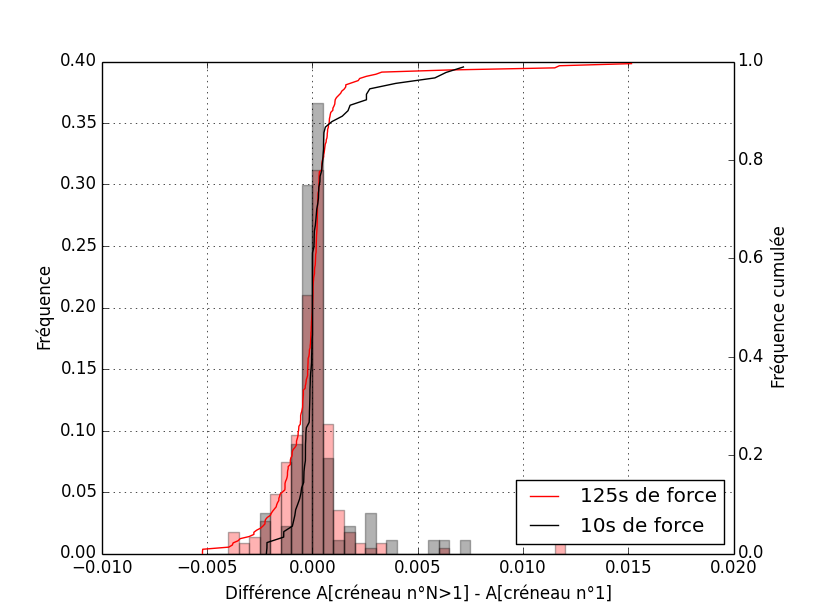
\includegraphics[scale=0.3]{Figures/A_diff.png} 
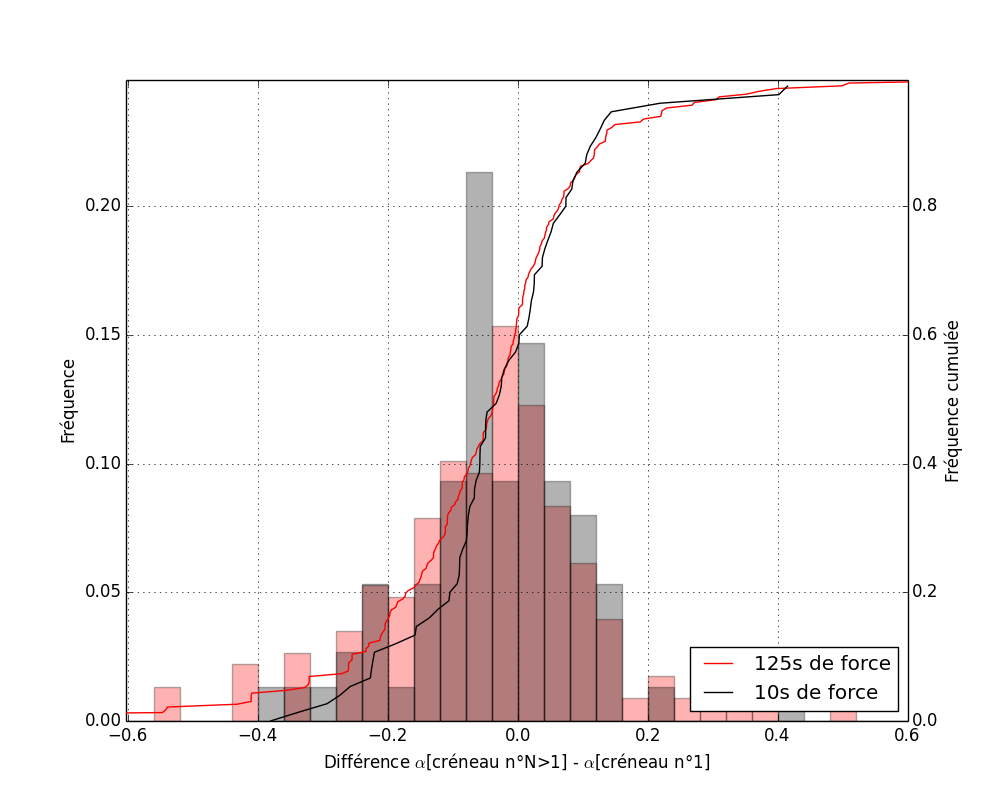
\includegraphics[scale=0.3]{Figures/E_diff.png}
\caption{Amplitude des évolutions entre la première mesure et les 6 suivantes, pour la série \no 3 témoin (en noir) et pour la même concentration de fibronectine et 125s de force en rouge.}
\label{Diff}

 
\end{figure}
On peut voir sur la figure \ref{Evolution_6c} qu'il n'y a pas de changements de $A$ communs à toute la population de cellules : ce ne sont pas toutes les cellules qui se rigidifient ou se ramollissent ensemble. 
En revanche, on peut observer un décalage des exposants vers les valeurs les plus faibles aux 2\ieme  et 3\ieme créneaux, qui se résorbe ensuite, mais il n'est pas significatif. 
Le comportement mécanique de ces cellules soumises à une force pendant de longues durées évolue donc d'abord dans le sens d'une \og élastification \fg , d'une diminution de la part dissipative de la réponse mécanique. 

Lorsque l'on applique une force pendant 125 secondes, l'amplitude des variations par rapport à la mesure d'origine de $A$ et $\alpha$ se détache du bruit obtenu pour seulement 10 secondes de forces, comme on peut le voir sur l'histogramme \ref{Diff}. L'application d'une force pendant une durée plus longue permet donc de modifier significativement les paramètres $A$ et $\alpha$. 

\subsection{Classification des cellules selon leur évolution}

Il n'y pas de tendance d'évolution de la population de cellules sondée au cours du temps, cependant on peut observer au niveau individuel l'évolution de $A$ pour en déduire une tendance au ramollissement ou à la rigidification. 

On classe ainsi les cellules en trois groupes : celles qui se rigidifient, avec $A$ décroissant significativement sur les 4 à 6 applications de force, celles qui se ramollissent $A$ croissant significativement sur les 4 à 6 applications de force, et celles qui n'ont pas une évolution significative ou cohérente dans le temps de $A$. 
On peut créer un classement semblable avec l'évolution de l'exposant $\alpha$. 
\begin{figure}
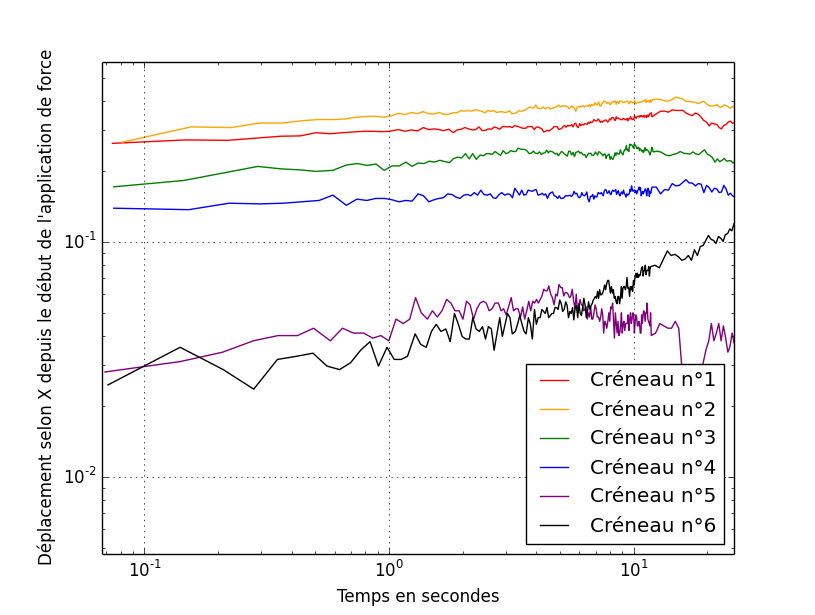
\includegraphics[scale=0.33]{Figures/Rigidification_exemple_s2c2.png} 
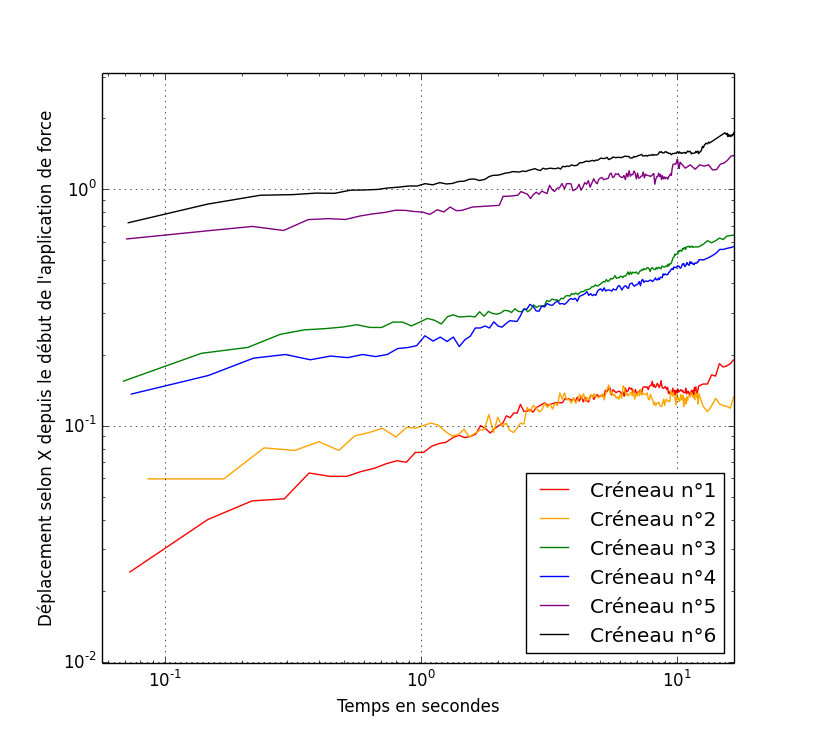
\includegraphics[scale=0.3]{Figures/Ramollissement_exemple_s2c19.png} 
\caption{Exemples de déplacements au cours du temps et au cours des applications de forces d'une cellule considérée comme en rigification (en haut) et d'une cellule en ramollissement (en bas). }
\end{figure}

\begin{figure}
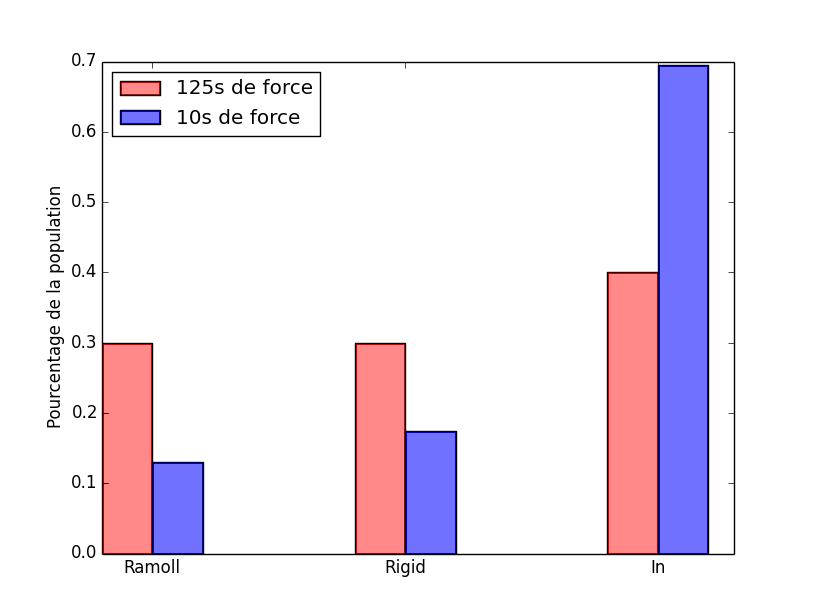
\includegraphics[scale=0.5]{Figures/FRI_temoin_vs_C4.png} 
\caption{Répartition des cellules dans les trois catégories d'évolution de $A$ au cours des applications de force \label{FRI_temoin}}
\end{figure}

On peut remarquer sur la figure \ref{FRI_temoin} que les cellules ont majoritairement un comportement incohérent lorsque la force n'est appliqué que durant 10 secondes.
Cette évolution aléatoire et de plus de faible amplitude comme on le voit sur la figure \ref{Diff} est très probablement le bruit sur la mesure de $A$. 

Lorsque la force est appliquée pendant 125 secondes, on peut au contraire observer qu'il y a beaucoup plus de cellules qui se ramollissent ou se rigidifient de manière persistante au cours du temps, avec une amplitude de variation plus grande que pour le témoin. 

\subsection{Influence de la position de la bille sur la cellule sur l'évolution des propriétés mécaniques}

On peut donc constater que parmi les cellules soumises à 125 secondes de force de manière répétée, 60\% ont une évolution cohérente de $A$ vers la rigidification ou le ramollissement et 40\% une évolution incohérente. 

Cette évolution dépend de la valeur initiale de $A$ : ce sont les cellules les plus molles initialement qui se rigidifient, et inversement. Mais cette dépendance est artificielle : les cellules déjà rigides qui se rigidifient n'ont pas de mouvement visible sur lequel faire des mesures, et les cellules molles qui se ramollissent finissent par voir leur bille arrachée, ou sortir du champ d'observation. 

Nous avons alors cherché si ces différences de comportement ne provenaient pas de la position de la bille sur la cellule, et de la direction selon laquelle on appliquait la contrainte. 

Il n'y pas de différence significative entre la distance dans le plan focal entre le bord de la bille et le bord du noyau (qui peut être négative si la bille est au-dessus du noyau) des trois différentes populations de cellules. 

Cependant, on peut observer que la position de la bille par rapport au noyau de la cellule, c'est-à-dire savoir si on tire la bille pour l'éloigner du noyau, ou pour la pousser vers le noyau, ou perpendiculairement à l'axe bille-noyau, est significativement différente pour les cellules ayant un comportement différent (testé avec un G-test d'indépendance). 
\begin{figure}
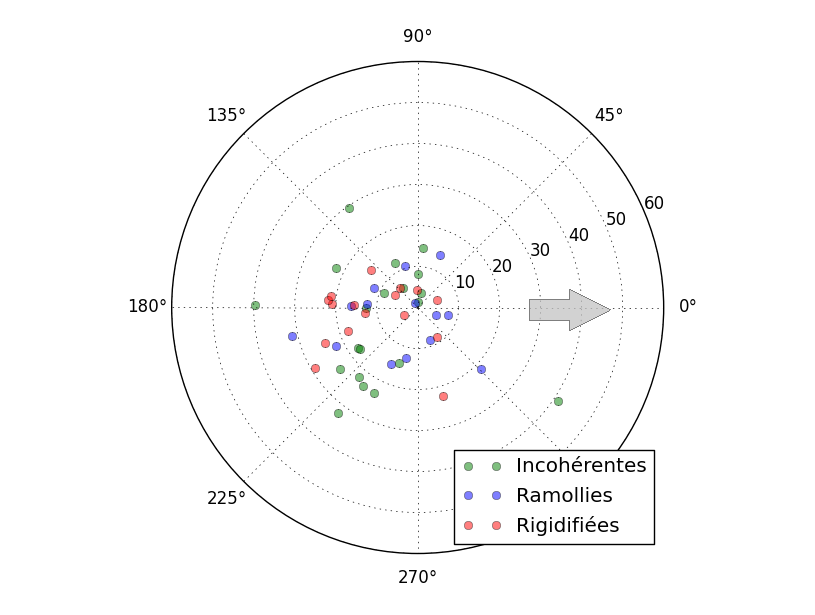
\includegraphics[scale=0.5]{Figures/Positions_FRI.png} 
\caption{Longueur et orientation du vecteur entre le bord du noyau et la bille. La flèche représente la direction de la force exercée sur les billes.}
\end{figure}
\begin{figure}
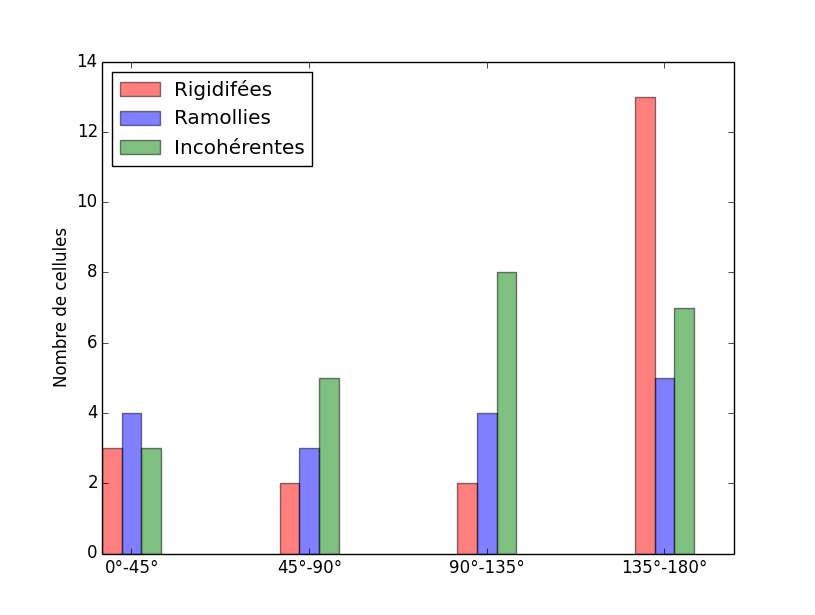
\includegraphics[scale=0.5]{Figures/Hist_Angles.png} 
\caption{Réparition des comportements cellulaires en fonction de l'angle formé entre l'axe bille-noyau et la direction de la force appliquée, pour 125 secondes de force et 4 \micro g de fibronectine. p=0.044 \label{Angle_C4}}
\end{figure}

En effet, 65\% des cellules rigidifiés sont du côté opposé à la direction de la force par rapport au noyau (leur angle est de plus de 135\degres ), alors que 57\% des cellules incohérentes ont un angle compris entre 45\degres et 135\degres . 
%\end{document}